\label{cha:grundlagen}
Als Fundament für die weitere Arbeit sollen zunächst eine Grundlagen erarbeitet werden. Um das Vorhaben und die Schritte dieser Arbeit besser nachvollziehen zu können, wird zunächst das Modell der \textit{Tetrade der Medieneffekte} vorgestellt. Hierbei handelt es sich um eine Idee von Marshall McLuhan, welcher sich über die Effekte welche ein Medium mit sich bringt. Er hat festgestellt, dass es sich hierbei um insgesamt vier Effekte handelt, welche er mit den folgenden Fragen bestimmen will \citep{mcluhan1977laws}:

\begin{enumerate}
\item What does the medium enhance?
\item What does the medium make obsolete?
\item What does the medium retrieve that had been obsolesced earlier?
\item What does the medium reverse or flip into when pushed to extremes?
\end{enumerate}

\todo[inline]{Um Inhalte (Beispiel aus Quelle), Überleitung zu den Abschnitten ergänzen, Verweis auf Kapitel Evaluation}

%Versuchen Sie dieses Konzept als Einleitung des Grundlagenteils zu adaptieren. Ich dem Leser (und Ihnen) kann es helfen, das Vorhaben besser einzuordnen. Wo kommen wir her, wo gehen wir hin und was kann noch alles daraus werden.

\section{Moodle}
\label{sec:moodle}
Bei Moodle (Modular Object-Oriented Dynamic Learning Environment) handelt es sich im Wesentlichem um eine frei verfügbares Open Source Learningmanagementsystem (GNU Public License) mit welchem Internet basierte Kurse entwickelt und durchgeführt werden können \citep{moodle2015was}. Ziel der Lernplattform ist es denen Lehrenden, Administratoren und Lernenden ein robustes, sicheres und integriertes System zu liefern, mit dessen Hilfe sie eine personalisierte Lernumgebung gestalten können \citep{moodle2018about}. Unter dieser Zielsetzung hat  Moodle weltweit als Lernplattform eine sehr weite Verbreitung und hat aktuell 101.447 registrierte Seiten in 232 Ländern mit insgesamt mehr als 130 Millionen Benutzern \citep{moodle2018stats}. Im Folgenden wird der Aufbau von einer Moodle Seite geschildert.

Zugriff auf Moodle erhält man über die Startseite, diese kann auf die eigenen Bedürfnisse angepasst werden. Auch kann Moodle so konfiguriert werden, dass die Startseite erst nach Anmeldung an der Login-Seite erfolgen kann. Die Grundstruktur von Moodle ist, wie in Abbildung \ref{fig:MoodleAufbau} zu sehen, anhand von Kursbereichen und Kursen organisiert. Kurse werden wiederum als Seiten repräsentiert, auf welchen die Lehrenden Arbeitsmaterialien und Aktivitäten für die Studierenden bereitstellen können. Kurse werden üblicherweise in einzelne Kursabschnitte unterteilt, in welchen die Arbeitsmaterialien und Aktivitäten eingebunden werden. Kursseiten können mittels Blöcken noch um weitere zusätzliche Informationen angereichert werden. Diese Kurse werden dann innerhalb von Kursbereichen organisiert. Hierbei ist auch ein mehrstufiges Kursbereichssystem umsetzbar \citep{moodle2015aufbau}.

\begin{figure}[h!]
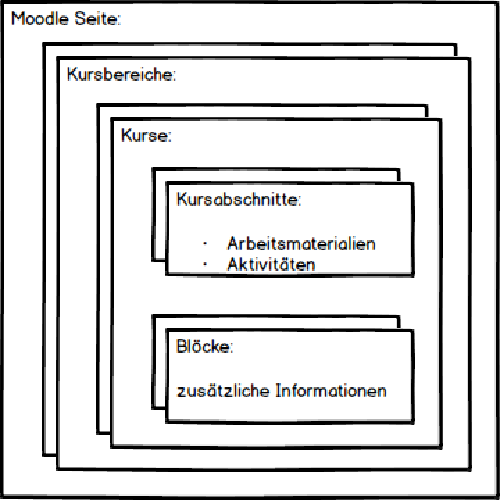
\includegraphics[width=.5\textwidth,center]{MoodleAufbau.pdf}
\caption{\label{fig:MoodleAufbau}Schematischer Aufbau einer Moodle Seite}
\end{figure}

Technisch baut Moodle auf den für eine Webanwendung üblichen Aufbau aus Webserver und Datenbank unter Verwendung von PHP auf. Um die zum Ziel gesetzt Personalisierbarkeit zu erreichen setzt auf Moodle unter anderem auf ein Plugin System. Jedes Plugin wird in einem von über 50 verschiedenen Plugin Typen einkategorisiert, jeder dieser Typen dient dazu einen speziellen Bereich von Moodle zu erweitern beziehungsweise anzupassen \citep{moodle2017plugin}.


%%%%%%%%%%
\section{Kooperation im Lernumfeld}
\dots
%Can a Hypermedia Cooperative e-Learning Environment Stimulate Constructive Collaboration?
%The efficacy of online cooperative learning systems
%Warum Kooperation neu erfinden? Zum Beitrag der CSCW-Forschung für das kollaborative E-Learning 

%%%%%%%%%%
\subsection{Offline}

%%%%%%%%%%
\subsection{Online}


%%%%%%%%%%
\section{Lernen mit Hypermedia}
Bevor wir uns der genauen Konzeption und Implementation des Moodle Plugins für Hyperaudio-Dokumente zuwenden, betrachten wir zunächst \textit{Hypermedia} im Allgemeinen. Dabei wollen wir zunächst eine Begriffsklärung durchführen. Darauf aufbauend werden einige Erfahrungen aus verschiedenen wissenschaftlichen Arbeiten gesammelt. Zuletzt wollen wir hieraus einige Rückschlüsse für unser Moodle Plugin und unsere Interpretation von Hyperaudio ziehen.

Hyperaudio stellt eine Ausprägung von \textit{Hypermedia} dar. Der Begriff \textit{Hypermedia} wurde das erste Mal von Ted Nelson 1965 verwendet \citep{nelson1965complex}. In seinem Paper beschreibt er detailliert, was er sich unter einem \textit{Hypertext} vorstellt. Hierunter versteht er ein Dokument bestehend aus geschriebenen oder bildhaften Inhalten, welche in solch einer komplexen Art und Weise miteinander verbunden sind, dass sie nicht mehr auf Papier dargestellt werden können. Es kann Zusammenfassungen, Karten über die Inhalte und deren Zusammenhänge, Annotationen, Ergänzungen oder Anmerkungen von Wissenschaftlern, die das Dokument begutachtet haben, enthalten. Nelson beschreibt das Kriterium für den Präfix \textit{hyper} damit, dass diese Objekte nicht durch eine Konvertierung in ein einfaches lineares Medium, wie beispielsweise einen String umgewandelt werden können. Der wesentliche Punkt ist also, dass es sich beim Lernen mit \textit{Hypermedia} um ein nicht-lineares Lernen handelt.

Genauer betrachtet stellt das, was Nelson sich damals als \textit{Hypertext} vorgestellt hatte, nach heutiger Definition bereits eine Form von \textit{Hypermedia} dar. Auch wenn viele die beiden Begriffe \textit{Hypertext} und \textit{Hypermedia} synonym verwenden \citep{nielsen2013multimedia}, werden bei strikter Betrachtung bei \textit{Hypertext} ausschließlich Texte miteinander verbunden, während bei \textit{Hypermedia} auch andere Medien eingebunden werden können. Gemeinsam haben beide Arten jedoch, dass der Lernende keinen linearen Weg vorgegeben hat, sondern von einem Knoten (Node) zum anderen springen kann und sich somit seinen Lernweg selbst aussucht. Als Folge dessen stellt \textit{Hypermedia} eine nicht-lineare Variante von \textit{Multimedia} dar.

Nach dieser Logik handelt es sich bei Hyperaudio in seiner klassischen Form eigentlich um reine Audiosequenzen, die miteinander verknüpft sind, wobei der Lernende selbst entschieden kann, in welcher Reihenfolge er diese abspielt \citep{zumbach2006learning}.

Wissenschaftler beschäftigen sich schon seit vielen Jahren damit, festzustellen, welche Effekte der Einsatz von \textit{Multimedia}, \textit{Hypertext} und \textit{Hypermedia} auf den Lernerfolg von Lehrenden hat. In der Arbeit von \cite{moos2010multimedia} wird eine Analyse von etlichen Arbeiten zu diesem Thema durchgeführt. \cite{moos2010multimedia} konzentrieren sich hierbei vor allem auf den Einfluss auf die Motivation der Lernenden. Dennoch wird auch auf andere Aspekte der drei verschiedenen E-Learning Methoden \textit{Multimedia}, \textit{Hypertext} und  \textit{Hypermedia} im Vergleich zu klassischen Lehrmethoden eingegangen.

\cite{moos2010multimedia} verweisen auf Arbeiten, nach denen eine Herausforderung bei \textit{Multimedia} und somit auch bei \textit{Hypermedia} darin besteht, dass die kognitive Aufnahmekapazität der Studierenden überschritten werden kann (Mayer und Moreno; van Merrienboer und Ayres, nach \cite{moos2010multimedia}), wenn Informationen sowohl aus einem Text als auch aus einem Diagramm entnommen werden sollen. Dies beruht auf der Annahme der Cognitive Load Theory, welche dem Arbeitsgedächtnis nur eine begrenzte Kapazität zuspricht (Sweller; van Merrienboer und Sweller, nach \cite{moos2010multimedia}). Es gibt aber auch Studien, welche einen positiven Effekt nachweisen, wenn zur gleichen Zeit Bilder dargestellt werden und dazu passender Text vorgelesen wird, im Vergeleich zum alleinigen Betracheten von Bildern beziehungsweise Anhören von Texten (Mayer und Anderson; Mayer und Sims, nach \cite{moos2010multimedia}).

\textit{Hypertext} bietet zwar Vorteile, da der Studierende den Lernweg bestimmen kann, der am besten auf seine Bedürfnisse angepasst ist. Auf der anderen Seite ist hierzu aber eine ausreichende Vorkenntnis in dem Lernbereich notwendig, um die Entscheidung, wie dieser Weg aussehen soll treffen zu können. Des Weiteren wirkt sich auch ein fehlendes Interesse des Studierenden negativ auf die Effektivität der \textit{Hypertext} Lernumgebung aus (Lawless und Kulikowich, nach \cite{moos2010multimedia}).
\todo[inline]{Zitat nochmals prüfen}

Es ist nun also nicht verwunderlich, dass \textit{Hypermedia} als Verschmelzung von \textit{Multimedia} und \textit{Hypertext} ebenfalls einige Herausforderungen mit sich bringt \citep{moos2010multimedia}. Scott und Schwartz (nach \cite{moos2010multimedia}) fordern für das Lernen mit \textit{Hypermedia} eine Balance zwischen effektiver Navigation und Inhaltsverständnis. Dies soll durch Prozesse zur Überwachung des eigenen Lernfortschritts erreicht werden, doch Untersuchungen haben ergeben, dass viele Studierende Schwierigkeiten haben diese Prozesse korrekt anzuwenden \citep{moos2010multimedia}.

\todo[inline]{Buch von Mayer}
\label{sec:audiocues}
\todo[inline]{Hyperaudio: Audio Cues - Donker}

Nachdem wir nun die Begrifflichkeiten um \textit{Hypermedia}, sowie den Begriff Hyperaudio im eigentlichen Sinne beleuchtet und entsprechende Studien betrachtet haben, gehen wir nun darauf ein, welche Rückschlüsse daraus für diese Arbeit gezogen werden können.

Zum einen stellen wir fest, dass wir den Begriff Hyperaudio nicht im ursprünglichen Sinn verwenden. Bei unseren Hyperaudio-Dokumenten handelt es sich eigentlich um Multimedia-Dokumente. Erst unter Berücksichtigung der Kommentarfunktion und der Galerie wird der Hypermedia-Aspekt erfüllt. Der Zuhörer hat also die Möglichkeit von Kommentar zu Kommentar oder von Annotation zu Annotation zu springen und gelangt dabei an die entsprechende Stelle in der Audiosequenz. In Ergänzung zu \cite{zumbach2006learning} verstehen wir unter Hyperaudio eine Audio-Datei, die durch die Erweiterung mittels Annotationen und Kommentarfunktion um Multimedia- und Hypermedia-Elemente ergänzt wird.

Der Vorteil unserer Betrachtungsweise von Hyperaudio liegt darin, dass die Herausforderungen, die in Verbindung mit \textit{Hypermedia} bzw. \textit{Hypertext} normalerweise auftreten, nicht besonders prägnant sind. In unserem Plugin wird dem Studierenden in erster Linie eine lineare Audio-Datei vorgespielt, die um Multimedia-Elemente ergänzt wird. Erst durch den Einsatz der Galerie und der Kommentarfunktion kommen die herausfordernden Elemente von Hypermedia ins Spiel. Dementsprechend sollte unser Hyperaudio-Plugin einen guten Kompromiss zwischen den verschiedenen Lehrmethoden darstellen.


%%%%%%%%%%
\section{Hyperaudio-Dokument}
\label{sec:hyperaudio}
\todo[inline]{Herleitung des Hyperaudio-Dokuments -> Entwicklung von Kurseinheit zu Hyperaudio -> Rückschluss auf Tetrade der Medieneffekte}
\todo[inline]{Nur Hyperaudio, nicht -Dokument. Dieser Abschnitt sollte m.E. früher, jedenfalls vor dem Lernen mit Multimedia, behandelt werden. }


%%%%%%%%%%
\section{Zusammenfassung}
\dots